% TODO: 目前内容不足以凑满两页(正反 A4 纸),所以有些内容注释掉了,之后完善

\documentclass{article}
\setlength\parindent{0pt}
\pagenumbering{gobble}

\usepackage{geometry}
\geometry{papersize={210mm,297mm}}
\geometry{left=9mm,right=9mm,top=9mm,bottom=9mm}

\usepackage{fontspec}
\setmainfont{DejaVu Sans}[Scale=0.9]

\usepackage{xeCJK}
\CJKfamily{zhsong}

\usepackage[svgcolors]{xcolor}
\usepackage{longfbox}
\usepackage{epstopdf}
\usepackage{float}
\usepackage{xpatch}
\usepackage{tipa}
\usepackage[export]{adjustbox}
\usepackage{enumitem}
\usepackage{mdframed}

\usepackage{multirow}
\usepackage{tabularx}
\renewcommand\tabularxcolumn[1]{m{#1}} % for vertical centering text in X column

\usepackage{multicol}
\usepackage[most]{tcolorbox}
\usepackage{amssymb}
\setlength{\columnsep}{3mm}

\usepackage[explicit,compact]{titlesec}
\titleformat{\section}{\normalfont\bfseries}{}{0pt}{【#1】}

% 啊!万能的 StackExchange!
% https://tex.stackexchange.com/questions/475466/latex-three-column-layout-merging-two-of-them-at-the-begining
%
\newlength{\abstractwidth}
\newlength{\columnshrink}
\newsavebox{\twocolinsert}
%
\makeatletter
\newlength{\resized@col}
\newcounter{column@count}
%
\xpatchcmd{\multi@column@out}{
	\process@cols\mult@gfirstbox{%
		\setbox\count@
		\vsplit\@cclv to\dimen@
		\set@keptmarks
		\setbox\count@
		\vbox to\dimen@
		{\unvbox\count@ \ifshr@nking\vfilmaxdepth\fi}%
	}%
}{
	\process@cols\mult@gfirstbox{%
		\global\advance\c@column@count\@ne
		\resized@col\dimen@%
		\ifnum\c@column@count=\tw@
				\advance\resized@col-\columnshrink
		\fi%
		\setbox\count@
		\vsplit\@cclv to\resized@col
		\set@keptmarks
		\setbox\count@
		\vbox to\dimen@{
			\ifnum
				\c@column@count=\tw@ \vspace*{\columnshrink}
			\fi
			\unvbox\count@
			\ifshr@nking\vfilmaxdepth\fi
		}%
	}%
}{\typeout{Success}}{\typeout{Failure}}
\makeatother

% for designing header
\newsavebox\mysavebox
\newenvironment{imgminipage}[2][]{%
   \def\imgcmd{\includegraphics[width=\wd\mysavebox, height=\dimexpr\ht\mysavebox+\dp\mysavebox\relax, #1]{#2}}%
   \begin{lrbox}{\mysavebox}%
   \begin{minipage}%
}{%
   \end{minipage}
   \end{lrbox}%
   \sbox\mysavebox{\setlength{\fboxrule}{0pt}\fbox{\usebox\mysavebox}}%
   \mbox{\rlap{\raisebox{-\dp\mysavebox}{\imgcmd}}\usebox\mysavebox}%
}

\renewcommand{\labelitemi}{$\blacktriangleright$}

\tcbset{
    frame code={}
    center title,
    left=0pt,
    right=0pt,
    top=6pt,
    bottom=0pt,
    colback=gray!40,
    colframe=white,
    enlarge left by=0mm,
    boxsep=0pt,
    arc=0pt,outer arc=0pt,
}

\begin{document}
\begin{multicols*}{3}

	\setlength{\abstractwidth}{2\linewidth}
	\addtolength{\abstractwidth}{\columnsep}
	\savebox{\twocolinsert}{\begin{minipage}{\abstractwidth}
		\noindent 核准日期:2025年04月19日
		\newline 修改日期:2025年04月19日,第一次修订
		\newline

		 \begin{mdframed}[leftline=false, rightline=false, innertopmargin=0pt, innerbottommargin=0pt, innerrightmargin=0pt, innerleftmargin=2em]
		 	\includegraphics[width=0.15\abstractwidth, valign=m]{assets/debian-text.eps}
		 	\hfill
		 	\begin{imgminipage}{assets/header-background.eps}[t]{0.7\abstractwidth}
		 		\Large \textbf{盒装安装媒介说明书}

		 		\normalsize 请仔细阅读说明书并在管理员指导下使用
		 	\end{imgminipage}
		 \end{mdframed}

		\includegraphics[width=\abstractwidth]{assets/header.eps}


		\begin{mdframed}[hidealllines=true, innerbottommargin=.5em, innertopmargin=0pt]
			\sffamily

			{\centering 警示语 \par}

			无论是否与其它操作系统合用,安装 Windows 均可能包含存在丢失磁盘上所有内容的各类风险。(参见【不良反应】)

			在使用 Microsoft Windows 时,您可能需要确认当前软硬件与当前 Windows 版本的兼容性。

			我们已确保大多数软硬件均可在最新  Microsoft Windows 下正常工作,但部分硬件或软件可能需要特定 Windows 系统分支、版本或兼容性策略的支持。
			
			若您使用了不支持的软件且未安装特定的兼容策略支持,严重时可能引发系统崩溃(BSOD)或造成不可挽回的数据丢失。
		\end{mdframed}
	\end{minipage}}
	\setlength{\columnshrink}{\ht\twocolinsert}
	\addtolength{\columnshrink}{\dp\twocolinsert}
	\noindent\usebox{\twocolinsert}


	\begin{tcolorbox}
	\section*{发行版名称}
	\end{tcolorbox}
	\begin{tabularx}{\linewidth}{@{}ll@{}}
		通用名称: & Windows \\
		正式中文名称: & 微软视窗操作系统 \\
		正式英文名称: & Microsoft Windows Operating System \\
	\end{tabularx}

	\medskip


	\begin{tcolorbox}
	\section*{内容}
	\end{tcolorbox}

	由美国微软公司开发的最新一代基于 Microsoft NT® 内核的操作系统。支持世界上绝大多数软件、硬件。内置各类基础软件。并为视觉正常的一般用户提供视觉生物友好型的 GUI 操作界面。同时为高级用户提供内置基于 Windows Console 或 Windows Terminal 的 PowerShell 或标准 cmd 命令行。并由美国微软公司提供各类其他操作系统的虚拟化运行支持。

	 内核版本:NT 10

	 版本号:“Sun Valley”

	\medskip


	\begin{tcolorbox}
	\section*{性质}
	\end{tcolorbox}

	本系统为采用 Microsoft NT® 内核的操作系统,安装后可由 UEFI 或 Legacy Compatible 引导方式启动。

	\medskip


	\begin{tcolorbox}
	\section*{适用平台}
	\end{tcolorbox}

	\begin{itemize}
		\item 支持使用 arm64、amd64、i686、ppc64el、mipsel、s390x 等架构的计算机、服务器和嵌入式设备。
		\item 本包装盒中的安装媒介适用平台以实际为准,一般为amd64平台。
	\end{itemize}


	\begin{tcolorbox}
	\section*{规格}
	\end{tcolorbox}

	1 枚 安装媒介

	\medskip

	\begin{tcolorbox}
	\section*{用法}
	\end{tcolorbox}

	使用 USB 设备引导。

	启动方式根据硬件调整,一般使用 UEFI。您也可以使用 Legacy Compatible 启动。

	根据硬件性能和个人需要,调整安装方式:一般而言,您将使用图形化界面进行安装;否则选择基于 Windows Terminal 命令行下的无 GUI 安装。

	安装好基本系统并设置完成 Microsoft Account 后,即可开始使用 Windows。

	\medskip

	\begin{tcolorbox}
	\section*{不良反应}
	\end{tcolorbox}

	Microsoft 有一个对用户和开发者所遇到的大多数 Microsoft Windows 软件、硬件以及 Windows 系统本身的问题的资料库。提供大量一般性问题与解决问题的操作步骤的解答。

	可以在 https://answers.microsoft.com 或 https://learn.microsoft.com 处获得它们。

	\medskip


	\begin{tcolorbox}
	\section*{注意事项}
	\end{tcolorbox}
	\begin{itemize}[leftmargin=*]

		\item 满足最低的硬件要求

		一枚 1 GHz 或更快的支持 64 位的处理器(双核或多核)或系统单芯片 (SoC) 对于 Microsoft Windows 而言是必须的。

		{\small\begin{tabularx}{\linewidth}{|X|X|X|X|}
			\hline
			类别 & RAM\newline (最低) & RAM\newline (推荐) & 硬盘 & 显卡 \\
			\hline
			有桌面 & 4GB & 8GB & 64GB & 支持 DirectX 12 或更高版本与 WDDM 2.0 驱动程序。 \\
		\end{tabularx}}

		基于您的需求,也许可以使用低于上表所列的配置完成系统安装。但我们无法保证安装后使用正常。

		\item 需要固件的设备

		Windows 会于安装完毕并接入互联网后自动安装所需的外部设备驱动程序,但部分硬件在使用之前可能需要更新固件(firmware)或微码(microcode)。

		部分不支持 UPnP (即插即用,Plug & Play)的硬件可能需要自行准备其他安装介质共同使用,并查阅相关说明安装使用。

	\end{itemize}


	\begin{tcolorbox}
	\section*{禁忌}
	\end{tcolorbox}

	在操作过程中出现或即将出现下列任何一种情况,请立即停止操作,并准备好系统恢复或软硬件维护。

	\begin{itemize}[leftmargin=*]
		\setlength{\itemsep}{0pt}
		\setlength{\parskip}{0pt}
		\setlength{\parsep}{0pt}

		\item 以任意管理员权限用户身份对C:/Widnows目录下执行删除操作。
		\item 未确认 ESP 分区所在磁盘号进行 ESP 分区修复。
		\item 未确认磁盘号执行低级格式化
		\item 令未经许可的个体对计算机进行操作且不进行监管
		\item 未经确认即执行来自非可信源的脚本或任意可执行文件
		\item 未经确认即开放高风险的可访问端口并关闭 Windows 防火墙
		\item 未经确认即自行修改有风险的注册表项目且未备份
		\item 长期在散热不良的设备上高负载使用
	\end{itemize}


	\begin{tcolorbox}
	\section*{无障碍安装}
	\end{tcolorbox}

	Microsoft Windows 安装介质一般情况下可在监护人陪同指导下,对视力或运动障碍人士使用。

	\medskip

	\begin{tcolorbox}
 	\section*{新手安装}
 	\end{tcolorbox}

	 Microsoft Windows 应谨慎用于新手安装,需要在管理员指导下进行安装,且需要定期进行密切的系统监测,一旦出现系统完整度或安全性的变化,应考虑停止使用 Microsoft Windows 并咨询相关管理员。

	% \medskip


	% \begin{tcolorbox}
	% \section*{版本迭代}
	% \end{tcolorbox}


	\begin{tcolorbox}
	\section*{系统相互作用}
	\end{tcolorbox}
	\begin{itemize}[leftmargin=*]
		\setlength{\parindent}{0pt}

		\item 与 Linux 的相互作用

		当您有双引导时,若 Linux 系操作系统与 Windows 访问相同的文件系统,则可能会导致问题和数据丢失。在这种情况下,文件系统的真实状态可能与 Windows 认为在“启动”之后的情况不同,并且可能在进一步写入文件系统时导致 Windows 默认不支持的文件系统损坏。因此,在双引导设置中,为了避免文件系统损坏,有必要在 Windows 中禁用“快速启动”功能。

		在罕见情况中已观察到,在使用 Windows 进行系统更新时,可能会出现重新启动后 GRUB 引导被破坏从而导致 Liunx 系操作无法启动的情况。同时,若在安装过程中将 Linux 系操作系统引导信息写入与 Windows 所在的物理磁盘 MBR 内,将导致后者无法正常启动。

		\item 与其他(不包括上述 Linux 系操作系统)操作系统的相互作用

		尚不明确。

		\item 与多个不同版本的 Windows 操作系统的相互作用
		
		一般情况下,您可以在一个硬盘上的多个分区或多个独立硬盘的不同分区上安全安装多个 Windows 操作系统。但部分涉及 ESP 分区修改的软件可能会不正确的将其他硬盘中的 Windows 引导信息进行错误修复,导致被错误修改的硬盘中的引导信息失效。严重时可能无法启动此 Windows 系统。因此,在进行 ESP 分区修改或引导修复前,请务必确认更改/修复的 ESP 分区正确。

		\item 与部分硬件的兼容性相互作用
		
		对于 Intel 13,14 酷睿处理器,当您使用“高性能”或更激进的电源计划时,可能会导致部分主板 BIOS 未更新至最新 Intel  0x12B 微码(Microcode)的处理器试图使用更高的电压来保持运行稳定。严重情况下可能会导致处理器产生“电子迁移”现象并需要更高电压以保持频率稳定,或称缩缸。因此,在使用13,14代 Intel 酷睿处理器时,请务必更新主板 BIOS 微码到 Intel 0x12B 或以上版本。

	\end{itemize}


	\begin{tcolorbox}
	\section*{贮藏}
	\end{tcolorbox}

	-40℃\textasciitilde +70℃

	请妥善贮藏所有安装媒介。
	
	建议贮藏于阴凉干燥处,避免阳光直射或暴露于电离辐射下。
	
	勿使不会安装 Microsoft Windows 的人员及儿童触及安装媒介、即便是安装完成后的操作系统亦是如此。

	\medskip


	\begin{tcolorbox}
	\section*{包装形式}
	\end{tcolorbox}

	装有 Microsoft Windows 安装镜像的、兼容 USB 3.0/2.0、SATA,NVMe M.2 协议的各类大容量存储设备。

	1 枚/盒

	\medskip


	\begin{tcolorbox}
	\section*{有效期}
	\end{tcolorbox}

	Microsoft Windows 已于 SQL Server 2017 开始,不再发布一切独立 Service Pack 支持更新并将其纳入到固定生命周期策略中。

	对于目前新式 Windows 生命周期终止支持之前,微软将至少提前 12 个月通知。
	
	现代 Microsoft Windows 每大版本更新支持至少为2年。大版本支持结束后,如非特殊情况不再发布任何相关更新。

	\medskip


	\begin{tcolorbox}
	\section*{执行标准}
	\end{tcolorbox}
	\begin{tabularx}{\linewidth}{@{}ll@{}}
		\multirow{4}{*}{}{使用条款:} & Microsoft TOU(Terms-of-use)\\
		~ & 以及其他授权条款。对于Microsoft TOU,您可以在https://www.microsoft.com/zh-cn/legal/terms-of-use 下获取相关内容。 \\
	\end{tabularx}

	\medskip


	\begin{tcolorbox}
	\section*{批准文号}
	\end{tcolorbox}

	本说明书使用 CC-BY-SA 3.0 协议授权。

	本再创作由公民北极星进行修改并遵守 CC-BY-SA 3.0 协议授权。感谢 @moesoha 提供原 repo。
	\medskip


 	\begin{tcolorbox}
 	\section*{生产单位}
 	\end{tcolorbox}

 	美国微软®公司

 	\medskip


	\begin{tcolorbox}
	\section*{说明书}
	\end{tcolorbox}
	\begin{tabularx}{\linewidth}{@{}ll@{}}
		\multirow{2}{*}{}{原编审:} & @YukariChiba\\
		~ & @moesoha \\
		原图形: & @YJBeetle\\
		现版本图形: & @SakuraRK (公民北极星_Official)\\
		GitHub: & moesoha/debian-media-box\\
	\end{tabularx}

	\medskip


	\vfill
	\begin{flushright}
		 - \linebreak 2021
		\linebreak
		\newline
		\begin{minipage}{0,5\textwidth}
			\centering
			$\vcenter{\hbox{
\includegraphics[height=10mm]{assets/microsoft-logo.eps}}}$
			$\vcenter{\hbox{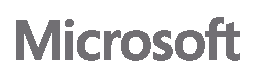
\includegraphics[height=5mm]{assets/microsoft-text.eps}}}$
		\end{minipage}
	\end{flushright}

\end{multicols*}
\end{document}
